\documentclass{article}
\usepackage{mathtools}
\usepackage{parskip}
\usepackage{graphicx}
\usepackage{mhchem}
\usepackage[flushmargin]{footmisc}
%\usepackage{fontspec}
%\usepackage{microtype}
\numberwithin{equation}{section}
\frenchspacing
%\setmainfont{Hoefler Text}
\begin{document}
\renewcommand{\thefootnote}{\fnsymbol{footnote}}
%\maketitle

\section{Introduction}

\textsc{Author's Note}: The following section contains what I hope is the essential background to get an unfamiliar reader up to speed and provide context on the topic of ligand-binding and cooperativity as it pertains to this work. Many of the nuances will be detailed in later sections and supported with models. Several treatises are available on this topic, and the reader is directed to them if more in-depth background is desired [klotz, wyman gil].

\subsection{Ligand Binding and Cooperativity}

The complex biochemical processes that give rise to life depend on the recognition of one molecule by another: a hormone binding to its receptor, an enzyme binding its substrate, a transcription factor binding \textsc{dna}, etc. A receptor recognizes its ligand, conventionally the smaller molecule, through non-covalent interactions comprising electrostatic forces, van der Waals forces, and the hydrophobic effect. The degree of recognition or \emph{affinity} of the receptor for its ligand is determined by the strength and number of non-covalent interactions between them, and those in turn are determined by the structure and chemical composition of the molecules, e.g., the type and spatial configuration of amino acids at the binding site of receptor protein. Analyses of ligand-receptor systems focus on affinity as the system's characteristic property and quantify it with the equilibrium constant of the binding reaction. A larger association constant = higher affinity, assoc constant also relates to range of concentrations or ligand binding interval, in class systems this is rouhgly 2 log units and we will see how this varies...

\begin{equation}
\ce{R + L <=> RL}\
\end{equation}

\begin{equation}
	\frac{\text{[RL]}}{\text{[R][L]}} = K_a
\end{equation}

\begin{equation}
	\bar{\nu} = \frac{\text{[bound ligand]}}{\text{[total receptor]}}
\end{equation}

\begin{equation}
	\bar{\nu} = \frac{\text[RL]}{\text{[R]+[RL]}} = \frac{K_a \text{[L]}}{1+K_a \text[L]}
\end{equation}

\begin{figure}
	\centering
	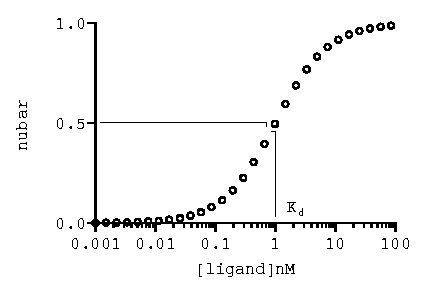
\includegraphics{iostherm_arrows}
\end{figure}

Differences in the magnitude of affinity are why a given receptor binds one ligand versus another. For example, an estrogen receptor will bind the hormone estrogen and effect a cellular change, but that same receptor will be unaffected by a another hormone such as insulin. This is because the structure and composition of the binding site on the receptor are complementary to those of the ligand and enable the formation of sufficient non-covalent interactions. Estrogen and insulin differ significantly in structure and composition (one is a steroid and the other a peptide) hence insulin cannot interact favorably with the binding site on the estrogen receptor. The converse is also true that a ligand will have a greater affinity if it can participate in additional or stronger interactions. This applies to receptors as well, where structural and compositional differences of binding sites account for differences in affinity. These phenomena have important implications when recalling a protein has conformational flexibility and can take on structural changes.

Consider a receptor with multiple binding sites for the same ligand. If the sites are structurally and compositionally the same, then we expect them to have the same affinity. However, if the structure changes, so will the nature of the interactions with the ligand and subseqently the affinity. In some receptors, a ligand can induce conformational changes when it binds and consequently modify affinity at another site. Depending on whether the affinity increases or decreases, the system is said to exhibit positive or negative cooperativity.\footnote{Cooperativity can be further classified as homotropic if the affinity is changed for an identical ligand (as explained) or heterotropic if the affinity is changed for a different ligand. In this work, cooperativity will always refer to homotropic cooperativity.} 

Cooperativity functions as a modulator of biochemical processes by shrinking or expanding the range of concentrations over which a receptor will bind its ligand. The classic example of this is the binding of oxygen by hemoglobin. Positive cooperativity in that system narrows the binding interval for oxygen so that it is efficiently transported from higher concentrations in the lungs to lower concentrations in tissues. Systems exhibiting positive cooperativity approach a switch-like state where the sites on the receptor   In systems exhibiting negative cooperativity, the ligand binding interval is expanded, could be considered a damping effect

We will see that it is imoprtants in signaling systems, but really what we need are appropriate models to study it



Negative cooperativity plays as role as we will see in some receptor systems --- response damped


For receptor proteins involved in cell signaling, modulation is an important component. Variations in affinity under different conditions. Dimerizing systems, blach blach

Dimerization, protein-protein interactions can be treated as a ligand-binding

We will see that EGFR exhibits negative coop and estrogen receptor exhibits pos coop but it also is a dimerizing system

Models to study cooperativity

This can be extended across multiple ligands or sites...and other disclaimers

\subsection*{Models: Visualizing Affinity}

\begin{equation}
	\text{R} + \text{L} \leftrightarrow \text{RL}
	\end{equation}
 












\end{document}